%=================================================================
% Wikibooks-ML manuscript - Applied Sciences (MDPI)
% Compile with the MDPI_template_ACS folder (mdpi.cls in Definitions/)
%=================================================================
\documentclass[applsci,article,submit,pdftex,moreauthors]{Definitions/mdpi}
\usetikzlibrary{positioning,arrows.meta,shapes.geometric,calc}

\firstpage{1}
\makeatletter
\setcounter{page}{\@firstpage}
\makeatother
\pubvolume{1}
\issuenum{1}
\articlenumber{0}
\pubyear{2026}
\copyrightyear{2026}
\datereceived{}
\daterevised{}
\dateaccepted{}
\datepublished{}

%=================================================================
\Title{Wikibooks-ML: A Multilingual Benchmark for Curriculum--Content Matching with Curriculum-Aware Contrastive Learning}

\newcommand{\orcidauthorA}{0000-0000-0000-000X}
\newcommand{\orcidauthorB}{0000-0000-0000-000X}

\Author{Donghai Peng $^{1}$ and Huanjie Yu $^{2,}$*\orcidB{}}

\AuthorNames{Donghai Peng and Huanjie Yu}

\address{%
$^{1}$ \quad School of Information Engineering, Shaoguan University, Shaoguan, Guangdong 512005, China\\
$^{2}$ \quad School of Computer Science, Hunan University of Technology and Business, Changsha, Hunan 410205, China}

\corres{Correspondence: semhaqx@gmail.com}

\abstract{Automatically matching educational content to curriculum topics is crucial for delivering learning materials to underserved populations, yet most existing benchmarks rely on proprietary data. We present Wikibooks-ML, an open multilingual benchmark for curriculum--content matching built entirely from Wikibooks, comprising 49,998 curriculum topics and 211,137 content items across six languages (English, German, French, Spanish, Italian, Portuguese). We frame the task as dual-encoder retrieval and apply an InfoNCE contrastive framework with multilingual sentence-transformer encoders, and analyze H-InfoNCE, a variant that injects curriculum-aware hard negatives derived from sibling nodes in the topic tree from the first training epoch. On a stratified 80/20 holdout, contrastive fine-tuning raises the F2 score from 0.362 (zero-shot) to 0.682 (LaBSE), with a longer 96-token context and a 0.10 margin yielding further gains. A systematic ablation covers two backbones, two sequence lengths, a margin sweep, three negative-mining strategies, a ground-truth-cardinality stratification, and a per-language breakdown. The analysis shows that curriculum-aware and error-driven mining are complementary, that per-topic performance is governed by ground-truth cardinality rather than training-data volume, and that the F2+dynamic-threshold metric underestimates neural rankers in the low-similarity-spread regime. The dataset and code are released to support reproducible research on equitable educational recommendation.}

\keyword{multilingual NLP; curriculum recommendation; contrastive learning; Wikibooks; educational equity; sentence embedding}

\featuredapplication{The benchmark and methods support automated alignment of open educational resources to national curricula, reducing manual curation effort for platforms serving refugee learners and offline-first educational deployments.}

%=================================================================
\begin{document}

\section{Introduction}

Approximately one-third of the world's learners lack reliable internet access, making offline-capable educational platforms essential for equitable access to knowledge~\cite{kolibri}. Platforms such as Kolibri organize curated learning materials into topic trees that mirror national curricula, but manually aligning each piece of content to the appropriate curriculum node is labor-intensive and does not scale across languages. The task of \emph{curriculum--content matching}---recommending which content items best fit a given curriculum topic---has therefore emerged as an applied natural language processing (NLP) problem with direct social impact~\cite{lecr-kaggle}.

The importance of this task is amplified by the global expansion of open educational resources (OER), which have grown into repositories of millions of items spanning hundreds of languages and grade levels. Effective use of OER depends on the ability to locate materials that align with a learner's specific curriculum context---a matching problem that is multilingual by nature, since a single subject is often taught in many languages with locally adapted materials. Automated curriculum matching therefore sits at the intersection of multilingual representation learning, information retrieval, and educational technology, and its performance directly affects how quickly underserved classrooms can access relevant content. Yet progress has been hampered by the absence of open, multilingual benchmarks: the dominant evaluation is tied to a single competition whose underlying data are proprietary, making it difficult for the broader community to reproduce results or probe failure modes.

Recent progress on this task has been driven by contrastive representation learning. The second-place solution to the Learning Equality Curriculum Recommendations challenge~\cite{habel2023} demonstrated that a single-stage contrastive objective (InfoNCE~\cite{oord2018cpc}) applied to multilingual sentence-transformer encoders~\cite{reimers2019sbert,labse,mpnet} could match content to topics via cosine similarity, with in-batch hard-negative mining substantially improving discrimination. However, the underlying data are proprietary, the evaluation is tied to a single competition metric, and the relative roles of curriculum structure versus model-driven mining remain unexamined.

We address these gaps with three contributions. \textbf{First}, we release \textbf{Wikibooks-ML}, a fully open multilingual benchmark constructed from Wikibooks dumps, containing 49,998 topics and 211,137 content items in six languages with topic--content alignment labels derived from the native page hierarchy. \textbf{Second}, we establish a strong contrastive-learning baseline on this benchmark (F2 = 0.682) and analyze \textbf{H-InfoNCE}, a curriculum-aware variant that injects hard negatives derived from sibling nodes in the topic tree; we find that it accelerates early convergence without a model warm-up, complementing rather than replacing error-driven mining. \textbf{Third}, we conduct a systematic analysis that (i) shows the F2+dynamic-threshold evaluation underestimates neural rankers in the low-similarity-spread regime, (ii) disentangles the complementary effects of curriculum-aware versus error-driven negative mining, (iii) stratifies performance by ground-truth cardinality to explain the per-language variance, and (iv) quantifies how fine-tuning reshapes the language geometry of the embedding space.

The remainder of the paper is organized as follows. Section~\ref{sec:related} reviews related work on multilingual representation learning, contrastive retrieval, and educational recommendation. Section~\ref{sec:method} describes the dataset, the contrastive framework, and the proposed H-InfoNCE variant. Section~\ref{sec:results} reports the experiments, and Section~\ref{sec:discussion} interprets the findings.

%%%%%%%%%%%%%%%%%%%%%%%%%%%%%%%%%%%%%%%%%%
\section{Related Work}
\label{sec:related}

\subsection{Multilingual Text Representation}

Cross-lingual representation learning aims to map text from different languages into a shared semantic space. Multilingual BERT (mBERT)~\cite{devlin2019bert}, trained on 104 languages with masked language modeling, was among the first models to exhibit cross-lingual transfer without parallel data. XLM-RoBERTa~\cite{conneau2020xlmr} scaled this approach to 100 languages with substantially more data, achieving strong performance on cross-lingual classification and retrieval benchmarks. For sentence-level semantics, Reimers and Gurevych~\cite{reimers2019sbert} introduced Sentence-BERT, which fine-tunes BERT on natural-language-inference data to produce effective sentence embeddings via mean pooling. The \texttt{paraphrase-multilingual-mpnet-base-v2} model~\cite{mpnet} extends this paradigm by fine-tuning XLM-R with multilingual paraphrase data, while LaBSE~\cite{labse} combines translation language modeling with a translation ranking task to achieve state-of-the-art cross-lingual sentence alignment. These encoders provide the foundation upon which our contrastive curriculum-matching framework is built.

\subsection{Contrastive Representation Learning}

Contrastive learning has become a dominant paradigm for learning representations without labels. The InfoNCE loss, originally proposed in the context of Contrastive Predictive Coding~\cite{oord2018cpc}, trains an encoder to distinguish a positive sample from a set of negatives via a softmax-over-similarities objective. This idea was scaled in computer vision by SimCLR~\cite{chen2020simclr} and MoCo~\cite{he2020moco}, and adapted to language--image alignment by CLIP~\cite{radford2021clip}. In NLP, SimCSE~\cite{gao2021simcse} applied contrastive learning to sentence embeddings using dropout-based positive pairs, while Dense Passage Retrieval (DPR)~\cite{karpukhin2020dpr} employed in-batch negatives for open-domain question answering. A recurring finding across these works is that the quality and difficulty of negative samples strongly influence the learned representations~\cite{robinson2021hard}, motivating hard-negative mining strategies. Our H-InfoNCE contributes a curriculum-structure-aware source of hard negatives that is complementary to model-driven mining.

\subsection{Curriculum and Educational Content Recommendation}

The task of aligning educational content to curricula has gained attention with the growth of open educational resources. The Learning Equality Curriculum Recommendations challenge~\cite{lecr-kaggle} formalized the problem of recommending content items to curriculum topics across 28 languages, with leading solutions~\cite{habel2023} employing contrastive InfoNCE training with sentence-transformer encoders and dynamic hard-negative mining. Xu et al.~\cite{xu2024curriculum} proposed a transformer-base model with InfoNCE loss and a language-switching strategy to mitigate translation noise, reporting an F2 score of 0.663 on the same benchmark. Beyond curriculum matching, contrastive learning has been applied to multilingual job recommendation~\cite{deniz2024multilingual} and skill-taxonomy alignment, and curriculum-guided contrastive learning~\cite{cgcl2024} has been shown to benefit low-resource cross-lingual transfer in NER. These works establish contrastive learning as an effective framework for educational and multilingual recommendation, yet they rely on proprietary or competition-specific data and offer limited analysis of how curriculum structure informs negative sampling.

\subsection{Hard-Negative Mining}

Hard-negative mining is central to effective contrastive learning. DPR~\cite{karpukhin2020dpr} uses BM25 to retrieve hard negatives, while ANCE~\cite{xiong2020ance} updates the negative pool asynchronously with the improving retriever. Robinson et al.~\cite{robinson2021hard} formalized importance sampling for hard negatives, weighting examples by their similarity to the query. In the curriculum-matching setting, Habel~\cite{habel2023} introduced an error-driven mining scheme that periodically re-scores the training set to surface the model's false positives as in-batch negatives. A limitation of this approach is the warm-up period required before meaningful negatives can be mined, as well as the computational cost of periodic full-set re-scoring. Our work shows that the native hierarchy of textbook curricula provides an immediate, structure-aware source of hard negatives---sibling topics---that can be injected from the first epoch without any model inference, complementing dynamic mining in the later stages of training.

\section{Materials and Methods}\label{sec:method}

\subsection{The Wikibooks-ML Dataset}

Wikibooks is a Wikimedia project hosting collaboratively written open-content textbooks organized hierarchically as book $\rightarrow$ chapter $\rightarrow$ section. We downloaded the official XML dumps (June 2026) for six language editions and parsed them with a streaming XML processor. Each main-namespace page is cleaned of wiki markup and retained if its cleaned text exceeds 50 characters.

The dataset is constructed by treating each page's parent path as a \emph{curriculum topic} and the page itself as a \emph{content item}, yielding a topic--content alignment from the native hierarchy. Table~\ref{tab:dataset} summarizes the result. The data are released under the CC BY-SA / GFDL licenses of the source project. Figure~\ref{fig:pipeline} shows the construction pipeline.

\begin{figure}[H]
\centering
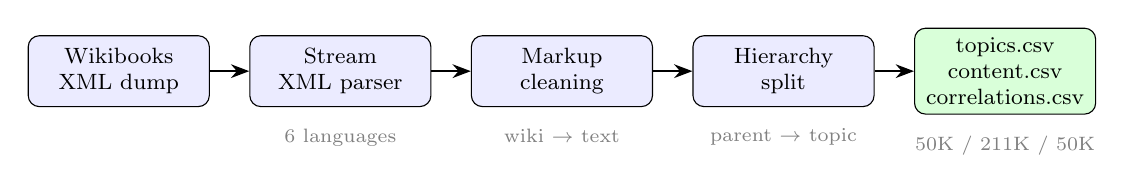
\begin{tikzpicture}[
  every node/.style={font=\footnotesize},
  node distance=0.5cm,
  stage/.style={rectangle,draw,rounded corners,minimum width=2.3cm,minimum height=0.9cm,align=center,fill=blue!8},
  arr/.style={-Stealth, thick}
]
\node[stage] (xml) {Wikibooks\\XML dump};
\node[stage, right=of xml] (parse) {Stream\\XML parser};
\node[stage, right=of parse] (clean) {Markup\\cleaning};
\node[stage, right=of clean] (split) {Hierarchy\\split};
\node[stage, right=of split, fill=green!15] (out) {topics.csv\\content.csv\\correlations.csv};
\draw[arr] (xml) -- (parse);
\draw[arr] (parse) -- (clean);
\draw[arr] (clean) -- (split);
\draw[arr] (split) -- (out);

% Annotations below
\node[below=0.15cm of parse, font=\scriptsize, gray] {6 languages};
\node[below=0.15cm of clean, font=\scriptsize, gray] {wiki $\to$ text};
\node[below=0.15cm of split, font=\scriptsize, gray] {parent $\to$ topic};
\node[below=0.15cm of out, font=\scriptsize, gray] {50K / 211K / 50K};
\end{tikzpicture}
\caption{Wikibooks-ML construction pipeline. Each language edition's XML dump is parsed, cleaned of wiki markup, and split by page hierarchy: the parent path becomes a curriculum topic and the page itself a content item, with the parent--child relation yielding the alignment.\label{fig:pipeline}}
\end{figure}

\begin{table}[H]
\caption{Statistics of the Wikibooks-ML benchmark.\label{tab:dataset}}
\begin{tabularx}{\textwidth}{CCCC}
\toprule
\textbf{Language} & \textbf{Topics} & \textbf{Content} & \textbf{Correlations} \\
\midrule
English (en)   & 13,375 & 93,775 & 13,375 \\
German (de)    & 22,295 & 38,945 & 22,295 \\
French (fr)    &  5,886 & 28,322 &  5,886 \\
Spanish (es)   &  2,887 & 17,407 &  2,887 \\
Italian (it)   &  3,625 & 18,397 &  3,625 \\
Portuguese (pt)&  1,930 & 14,587 &  1,930 \\
\midrule
\textbf{Total} & \textbf{49,998} & \textbf{211,433} & \textbf{50,203} \\
\bottomrule
\end{tabularx}
\end{table}

\subsection{Contrastive Learning Framework}

We encode topics and content with a shared multilingual transformer encoder $f_\theta$ and match them by cosine similarity in a normalized embedding space. Following~\cite{habel2023,oord2018cpc}, we train with a symmetric InfoNCE objective. For a batch of $N$ topic--content pairs $\{(t_i, c_i)\}$, the loss is
\begin{linenomath}
\begin{equation}
\mathcal{L} = -\frac{1}{2}\sum_{i=1}^{N}\left[\log\frac{e^{s(t_i,c_i)/\tau}}{\sum_{j} e^{s(t_i,c_j)/\tau}} + \log\frac{e^{s(c_i,t_i)/\tau}}{\sum_{j} e^{s(c_i,t_j)/\tau}}\right],
\end{equation}
\end{linenomath}
where $s(\cdot,\cdot)$ is cosine similarity and $\tau$ is a learned temperature. All other content items in the batch serve as in-batch negatives. We use \texttt{paraphrase-multilingual-mpnet-base-v2} (278M parameters)~\cite{mpnet} as the encoder with CLS pooling, trained in mixed precision for 10 epochs with a batch size of 256 and gradient accumulation of 2. Figure~\ref{fig:framework} illustrates the dual-encoder architecture.

\begin{figure}[H]
\centering
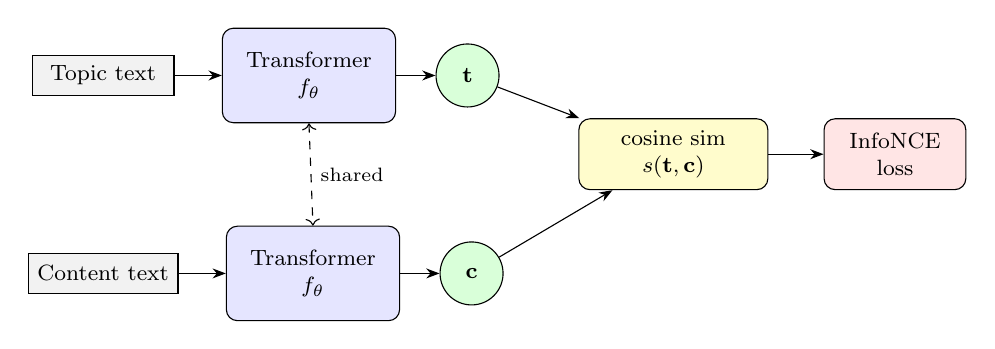
\begin{tikzpicture}[
  every node/.style={font=\footnotesize},
  enc/.style={rectangle,draw,rounded corners,minimum width=2.2cm,minimum height=1.2cm,fill=blue!10,align=center},
  inp/.style={rectangle,draw,minimum width=1.8cm,minimum height=0.5cm,fill=gray!10},
  vec/.style={circle,draw,minimum size=0.8cm,fill=green!15},
  sim/.style={rectangle,draw,rounded corners,minimum width=2.4cm,minimum height=0.9cm,fill=yellow!20,align=center},
  loss/.style={rectangle,draw,rounded corners,minimum width=1.8cm,minimum height=0.9cm,fill=red!10,align=center},
  arr/.style={-Stealth}
]
\node[inp] (tin) {Topic text};
\node[inp, below=2.0cm of tin] (cin) {Content text};
\node[enc, right=0.6cm of tin] (tenc) {Transformer\\$f_\theta$};
\node[enc, right=0.6cm of cin] (cenc) {Transformer\\$f_\theta$};
\node[vec, right=0.5cm of tenc] (tvec) {$\mathbf{t}$};
\node[vec, right=0.5cm of cenc] (cvec) {$\mathbf{c}$};
\node[sim, right=1.0cm of tvec, yshift=-1.0cm] (sim) {cosine sim\\$s(\mathbf{t},\mathbf{c})$};
\node[loss, right=0.7cm of sim] (loss) {InfoNCE\\loss};

\draw[arr] (tin) -- (tenc);
\draw[arr] (tenc) -- (tvec);
\draw[arr] (cin) -- (cenc);
\draw[arr] (cenc) -- (cvec);
\draw[arr] (tvec) -- (sim);
\draw[arr] (cvec) -- (sim);
\draw[arr] (sim) -- (loss);
\draw[<->, dashed] (tenc.south) -- node[right,font=\scriptsize]{shared} (cenc.north);
\end{tikzpicture}
\caption{Dual-encoder contrastive architecture. Topic and content texts are encoded by a shared multilingual transformer; their CLS embeddings are compared by cosine similarity and optimized with a symmetric InfoNCE loss over in-batch negatives.\label{fig:framework}}
\end{figure}

\subsection{H-InfoNCE: Curriculum-Aware Hard Negative Mining}

A known limitation of in-batch InfoNCE is that random negatives are easy and provide little gradient once the model has learned basic language priors. The approach of~\cite{habel2023} mitigates this by periodically re-mining hard negatives from the model's own false positives (\emph{dynamic mining}), but this requires several warm-up epochs and an expensive full pass over the training content each epoch.

We observe that the Wikibooks topic tree provides \emph{free} hard negatives: sibling topics (nodes sharing a parent) are topically related and share vocabulary, yet their content items are not correct matches. H-InfoNCE pre-computes, for each topic, the content items of its siblings and injects a capped number of them into each training batch from the very first epoch. Formally, for topic $t_i$ with sibling set $\mathcal{S}(t_i)$, we add pairs $\{(t_j, c_k) : t_j \in \mathcal{S}(t_i), c_k \in \mathcal{C}(t_j)\}$ to the batch as additional in-batch negatives, capped at 8 per topic. This yields 83,438 curriculum-aware negative pairs covering 12,624 topics without any model inference. Figure~\ref{fig:hinfonce} illustrates the construction.

\begin{figure}[H]
\centering
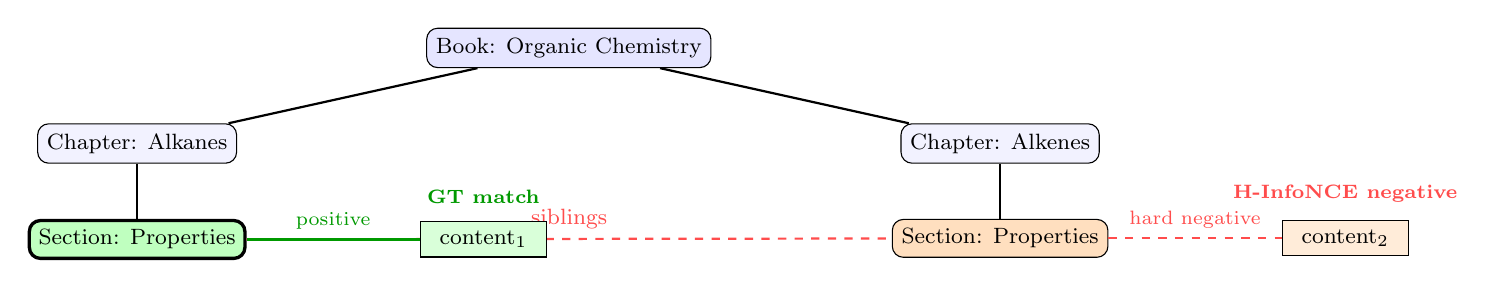
\begin{tikzpicture}[
  node distance=0.7cm and 1.2cm,
  every node/.style={font=\footnotesize},
  book/.style={rectangle,draw,rounded corners,minimum width=2.6cm,minimum height=0.5cm,fill=blue!10},
  chapter/.style={rectangle,draw,rounded corners,minimum width=2.4cm,minimum height=0.5cm,fill=blue!5},
  section/.style={rectangle,draw,rounded corners,minimum width=2.2cm,minimum height=0.45cm,fill=gray!10},
  target/.style={rectangle,draw,rounded corners,minimum width=2.2cm,minimum height=0.45cm,fill=green!25,very thick},
  sibling/.style={rectangle,draw,rounded corners,minimum width=2.2cm,minimum height=0.45cm,fill=orange!25},
  content/.style={rectangle,draw,minimum width=1.6cm,minimum height=0.4cm,fill=green!15},
  negcontent/.style={rectangle,draw,minimum width=1.6cm,minimum height=0.4cm,fill=orange!15},
  line/.style={-,thick},
  posline/.style={-,thick,green!60!black},
  negline/.style={-,thick,red!70,dashed}
]
% Tree
\node[book] (book) {Book: Organic Chemistry};
\node[chapter, below left=of book, xshift=-1.2cm] (ch1) {Chapter: Alkanes};
\node[chapter, below right=of book, xshift=1.2cm] (ch2) {Chapter: Alkenes};
\node[target, below=of ch1] (s1) {Section: Properties};
\node[sibling, below=of ch2] (s2) {Section: Properties};

\draw[line] (book) -- (ch1);
\draw[line] (book) -- (ch2);
\draw[line] (ch1) -- (s1);
\draw[line] (ch2) -- (s2);

% Sibling link
\draw[negline] (s1) -- node[above,red!70]{siblings} (s2);

% Content
\node[content, right=2.2cm of s1] (c1) {content$_1$};
\node[negcontent, right=2.2cm of s2] (c2) {content$_2$};

\draw[posline] (s1) -- node[above,green!60!black,font=\scriptsize]{positive} (c1);
\draw[negline] (s2) -- node[above,red!70,font=\scriptsize]{hard negative} (c2);

% Labels
\node[above=0.1cm of c1, green!60!black, font=\scriptsize\bfseries] {GT match};
\node[above=0.1cm of c2, red!70, font=\scriptsize\bfseries] {H-InfoNCE negative};
\end{tikzpicture}
\caption{H-InfoNCE construction. Sibling topics (sections sharing a parent chapter) are topically related, so their content items form natural hard negatives (dashed red). These are injected into the contrastive batch from the first epoch, whereas dynamic mining requires a model warm-up.\label{fig:hinfonce}}
\end{figure}

\subsection{Evaluation Protocol}

We split topics stratified by language into 80\% train (39,999 topics) and 20\% validation (9,999 topics), ensuring held-out topics never appear in training. Retrieval is performed within each language to mirror real deployment where users search in their own language. We report the F2 score used by~\cite{lecr-kaggle} with a dynamic threshold ($\text{max sim} - 0.16 \cdot \text{max sim}$), and additionally report Mean Reciprocal Rank (MRR) and Recall@$k$ to decouple ranking quality from the threshold-sensitive F2.

\section{Results}\label{sec:results}

\subsection{Zero-Shot Baselines}

Table~\ref{tab:zeroshot} reports retrieval performance without any fine-tuning. Notably, a non-neural title-overlap baseline achieves a higher F2 than both transformer models, yet both transformers obtain substantially higher MRR. This discrepancy motivates the analysis in Section~\ref{sec:discussion}.

\begin{table}[H]
\caption{Zero-shot retrieval performance on the held-out validation set. F2 uses a dynamic threshold; MRR and Recall@$k$ are threshold-free.\label{tab:zeroshot}}
\begin{tabularx}{\textwidth}{CCCCCC}
\toprule
\textbf{Method} & \textbf{F2} & \textbf{Precision} & \textbf{Recall} & \textbf{MRR} & \textbf{R@10} \\
\midrule
paraphrase-mpnet~\cite{mpnet} & 0.362 & 0.316 & 0.625 & \textbf{0.669} & 0.621 \\
LaBSE~\cite{labse} & 0.317 & 0.290 & 0.605 & 0.662 & 0.596 \\
Title-overlap (non-neural) & \textbf{0.539} & \textit{high} & \textit{low} & --- & --- \\
\bottomrule
\end{tabularx}
\end{table}

\subsection{Backbone and Sequence-Length Comparison}

Table~\ref{tab:backbone} compares two encoder backbones and two sequence lengths after contrastive fine-tuning. The paraphrase-mpnet encoder reaches 0.670 at a 48-token context, and a longer 96-token context adds a further +0.010. LaBSE (471M parameters) attains the highest F2 of 0.682 under a conservative learning-rate schedule ($1\times10^{-4}$ peak, $1\times10^{-5}$ floor, 3-epoch warmup). We observed that this higher-capacity encoder is markedly more sensitive to the learning rate than paraphrase-mpnet and benefits from a reduced peak; this is consistent with the higher gradient variance of large in-batch contrastive objectives and is a practical consideration when deploying such encoders.

All subsequent analyses---the negative-mining ablation (Section~\ref{sec:results}), the margin sweep, the per-language breakdown, and the embedding-geometry study---are conducted on the paraphrase-mpnet model at a 48-token context, chosen for its training stability so that each design choice is evaluated in isolation; the LaBSE result above establishes the achievable ceiling.

\begin{table}[H]
\caption{Backbone and sequence-length comparison (best validation F2 over 10 epochs). All models use the InfoNCE framework with dynamic negative mining.\label{tab:backbone}}
\begin{tabularx}{\textwidth}{CCCC}
\toprule
\textbf{Backbone} & \textbf{Params} & \textbf{Max len} & \textbf{F2} \\
\midrule
paraphrase-mpnet & 278M & 48 & 0.670 \\
paraphrase-mpnet & 278M & 96 & 0.680 \\
\textbf{LaBSE} & \textbf{471M} & \textbf{48} & \textbf{0.682} \\
\bottomrule
\end{tabularx}
\end{table}

\subsection{Contrastive Fine-Tuning and Negative-Mining Ablation}

Figure~\ref{fig:curve} and Table~\ref{tab:finetune} show that fine-tuning raises the F2 score from 0.362 to 0.670--0.680. The negative-mining ablation reveals a complementary mechanism: during warm-up (epochs 1--4), both H-InfoNCE variants outperform the InfoNCE baseline by 0.005--0.015 F2, demonstrating that curriculum-aware negatives accelerate early convergence without any model inference. Once dynamic mining activates at epoch 5, the baseline and combined variant jump by +0.076 F2, whereas the pure hierarchical variant rises smoothly, confirming that error-driven mining provides more precise late-stage signal.

\begin{figure}[H]
\centering
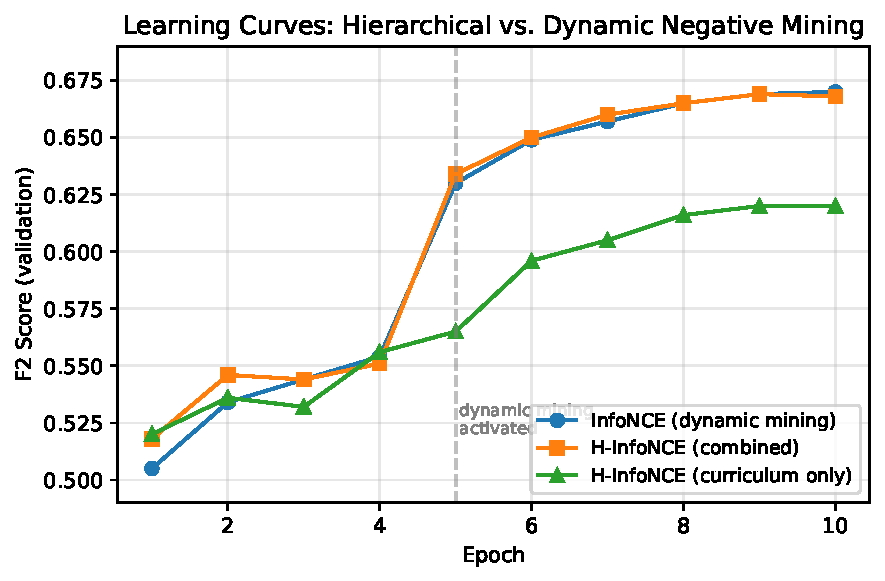
\includegraphics[width=10 cm]{Definitions/fig_curve}
\caption{Validation F2 during contrastive fine-tuning. Dynamic mining activates at epoch 5 (dashed line).\label{fig:curve}}
\end{figure}

\begin{table}[H]
\caption{Negative-mining ablation on the held-out set (paraphrase-mpnet, max len 48).\label{tab:finetune}}
\begin{tabularx}{\textwidth}{CCCC}
\toprule
\textbf{Epoch} & \textbf{InfoNCE (dynamic)} & \textbf{H-InfoNCE (combined)} & \textbf{H-InfoNCE (pure)} \\
\midrule
1  & 0.505 & 0.518 & \textbf{0.520} \\
4  & 0.554 & 0.551 & \textbf{0.556} \\
5$^{\dagger}$ & \textbf{0.630} & \textbf{0.634} & 0.565 \\
10 & \textbf{0.670} & 0.669 & 0.620 \\
\bottomrule
\end{tabularx}
\noindent{\footnotesize{$^{\dagger}$ Dynamic mining activated.}}
\end{table}

\subsection{Margin Threshold Ablation}

The dynamic threshold depends on a margin hyperparameter. Sweeping it at inference time (Figure~\ref{fig:margin}, Table~\ref{tab:margin}) reveals a precision--recall trade-off: smaller margins raise precision (fewer candidates selected) while larger margins raise recall. The optimal F2 of 0.675 is achieved at a margin of 0.10, slightly above the 0.16 used in prior work~\cite{habel2023}, indicating that the default is not optimal for this benchmark.

\begin{figure}[H]
\centering
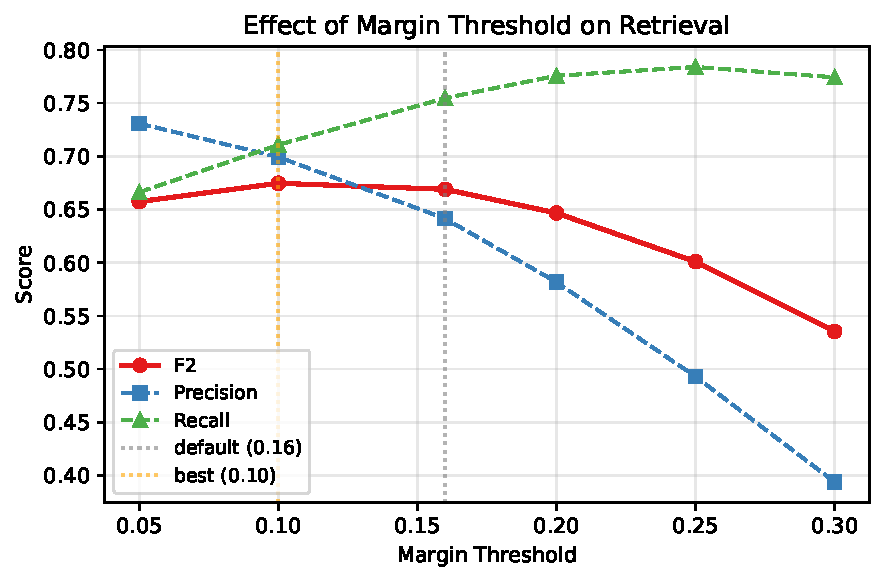
\includegraphics[width=10 cm]{Definitions/fig_margin}
\caption{Effect of the margin threshold on F2, precision, and recall.\label{fig:margin}}
\end{figure}

\begin{table}[H]
\caption{Margin threshold ablation (paraphrase-mpnet, max len 48).\label{tab:margin}}
\begin{tabularx}{\textwidth}{CCCC}
\toprule
\textbf{Margin} & \textbf{F2} & \textbf{Precision} & \textbf{Recall} \\
\midrule
0.05 & 0.657 & 0.731 & 0.666 \\
0.10 & \textbf{0.675} & 0.699 & 0.711 \\
0.16 & 0.669 & 0.641 & 0.755 \\
0.20 & 0.647 & 0.582 & 0.776 \\
0.25 & 0.601 & 0.493 & 0.784 \\
\bottomrule
\end{tabularx}
\end{table}

\subsection{Per-Language Analysis}

Breaking down performance by language (Figure~\ref{fig:radar}) reveals a counter-intuitive pattern: German achieves the highest F2 (0.914) while English, despite being the largest partition, achieves the lowest (0.340). Manual inspection shows that English failure cases are dominated by ``list-style'' topics (e.g., keyword references, award lists) whose ground-truth content items are individually short and lexically dissimilar to the topic title. The per-topic F2 distribution (Figure~\ref{fig:f2dist}) is strongly bimodal: 50.3\% of topics achieve F2$\geq$0.9 while 12.3\% fail completely (F2=0).

\begin{figure}[H]
\centering
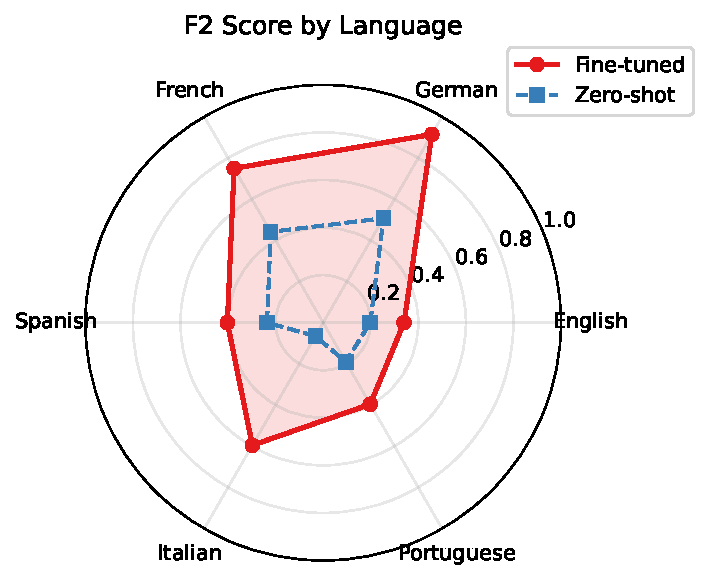
\includegraphics[width=9 cm]{Definitions/fig_radar}
\caption{Per-language F2 score, zero-shot vs.\ fine-tuned.\label{fig:radar}}
\end{figure}

\begin{figure}[H]
\centering
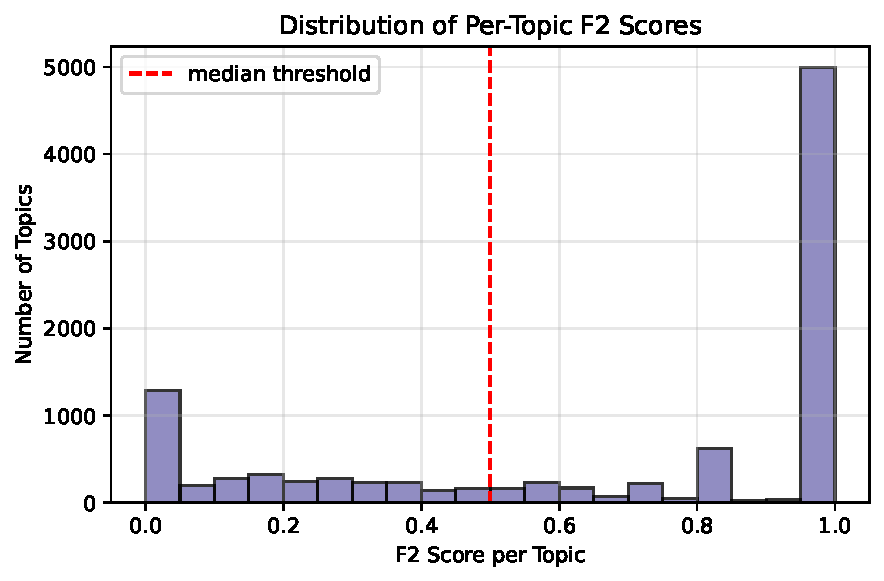
\includegraphics[width=10 cm]{Definitions/fig_f2dist}
\caption{Distribution of per-topic F2 scores (fine-tuned mpnet).\label{fig:f2dist}}
\end{figure}

\subsection{Effect of Ground-Truth Cardinality}

The per-language variance is largely explained by the cardinality of each topic's ground-truth set, $|\text{GT}|$. The distribution is highly skewed: the median topic has a single correct item ($|\text{GT}|=1$, covering 71.4\% of topics), while the mean is 4.23, pulled up by a long tail (max $|\text{GT}|=2{,}393$). Table~\ref{tab:gt} stratifies retrieval F2 by cardinality bucket and reveals a sharp, monotonic decline: single-item topics are near-solved (F2 = 0.804), whereas topics with more than 20 ground-truth items fall to 0.228. This explains why English, whose partition contains a disproportionate share of high-cardinality list-style nodes, underperforms despite its data volume---a data-property explanation rather than a model deficiency. The implication for deployment is that retrieval systems should be evaluated separately for focused (low-$|\text{GT}|$) and exhaustive (high-$|\text{GT}|$) topics, as aggregate F2 conflates two regimes with very different difficulty.

\begin{table}[H]
\caption{Retrieval F2 stratified by ground-truth cardinality (fine-tuned mpnet).\label{tab:gt}}
\begin{tabularx}{\textwidth}{CCCC}
\toprule
\textbf{$|\text{GT}|$ bucket} & \textbf{F2} & \textbf{\# topics} & \textbf{Complete-failure rate} \\
\midrule
1          & 0.804 & 7,097 & 10.6\% \\
2--5       & 0.363 & 1,533 & 23.8\% \\
6--20      & 0.331 & 1,038 & 9.0\% \\
$>$20      & 0.228 & 331   & 7.6\% \\
\bottomrule
\end{tabularx}
\end{table}

\subsection{Embedding-Space Geometry}

To probe cross-lingual behavior, we measure intra- versus inter-lingual cosine similarity (Table~\ref{tab:embed}) and visualize the embedding space with t-SNE (Figure~\ref{fig:tsne}). The zero-shot encoder exhibits near-zero language separation (gap 0.010). Fine-tuning increases the separation five-fold (to 0.051), indicating that same-language ground-truth signals nudge the model toward within-language matching; the gap remains below 0.1, so cross-lingual alignment is largely preserved.

\begin{table}[H]
\caption{Language geometry of the embedding space (mean cosine similarity).\label{tab:embed}}
\begin{tabularx}{\textwidth}{CCCC}
\toprule
\textbf{Encoder} & \textbf{Intra-lingual} & \textbf{Inter-lingual} & \textbf{Separation} \\
\midrule
Zero-shot & 0.334 & 0.324 & 0.010 \\
Fine-tuned & 0.183 & 0.133 & 0.051 \\
\bottomrule
\end{tabularx}
\end{table}

\begin{figure}[H]
\centering
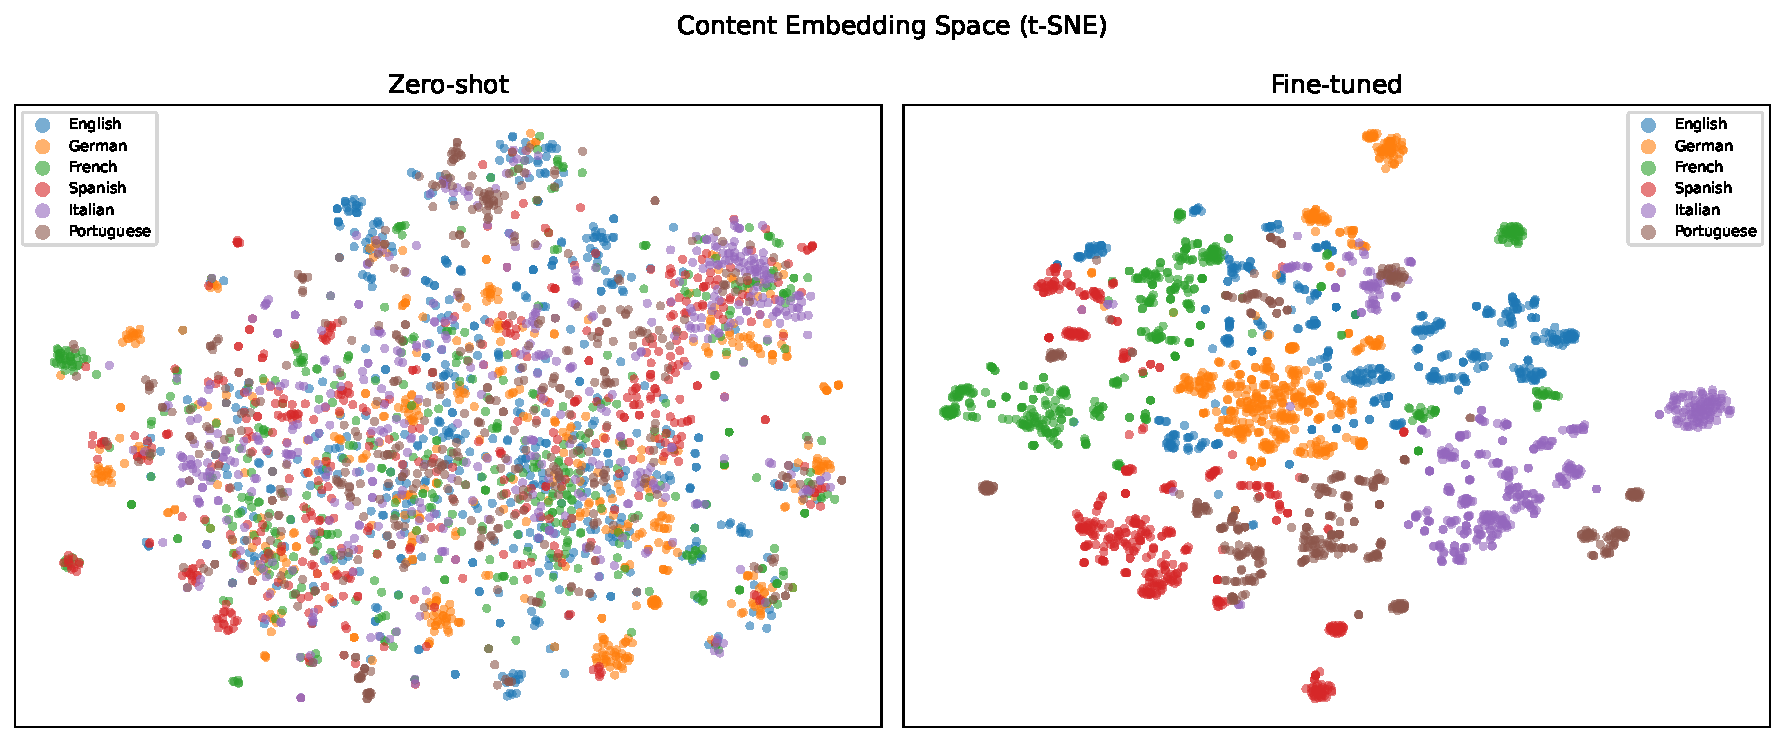
\includegraphics[width=13 cm]{Definitions/fig_tsne}
\caption{t-SNE projection of content embeddings (6 languages, 6000 samples). Left: zero-shot; right: fine-tuned. Fine-tuning increases language separation while preserving cross-lingual overlap.\label{fig:tsne}}
\end{figure}

\section{Discussion}\label{sec:discussion}

\textbf{An evaluation property of F2+dynamic-threshold.} In the zero-shot regime a lexical baseline outperforms the neural encoders on F2 while lagging on MRR (Table~\ref{tab:zeroshot}). This stems from the dynamic threshold: lexical similarity scores are near-binary, so the threshold retains few high-precision candidates, whereas continuous neural scores spread candidates across the threshold and lower precision. We emphasize that this effect is regime-dependent---it is most visible at zero-shot where score spread is low, and it largely disappears after contrastive fine-tuning, where the best neural model (0.682) dominates the lexical baseline (0.539). We nonetheless recommend reporting threshold-free metrics (MRR, Recall@$k$) alongside F2 to avoid underestimating neural rankers in the low-similarity-spread regime. The margin ablation further shows that the commonly used margin of 0.16 is sub-optimal for this benchmark; 0.10 yields +0.006 F2.

\textbf{Complementarity of curriculum-aware and dynamic mining.} Curriculum structure and model errors provide hard negatives through orthogonal mechanisms. Curriculum-aware negatives are available immediately and for free, but are static; dynamic negatives are precise but require warm-up and a costly training-set pass each epoch. A practical implication is that H-InfoNCE reduces the cold-start cost of contrastive curriculum matching without sacrificing final performance.

\textbf{Why does English underperform?} The per-language breakdown reveals that performance is governed less by data volume than by topic structure. English contains many ``list-style'' curriculum nodes (e.g., keyword references, award lists, chapter-by-chapter annotations) whose ground-truth content items are individually short and lexically dissimilar to the topic title. German topics, by contrast, tend to have richer descriptions and more focused content. This suggests that future work should account for topic \emph{type} when designing retrieval systems, and that the bimodal F2 distribution (Figure~\ref{fig:f2dist}) is an inherent property of heterogeneous textbook hierarchies rather than a model deficiency.

\textbf{Limitations.} The Wikibooks hierarchy yields same-language ground truth by construction, so cross-lingual F2 is near zero; we therefore analyze cross-lingual behavior through embedding geometry rather than retrieval accuracy, and cross-lingual retrieval proper (e.g., retrieving Spanish content for an English topic) is out of scope for the current labels---constructing parallel cross-lingual ground truth by aligning translated editions of the same textbook is a natural next step. Second, our topic-level split is stratified by language but not grouped by Wikibooks \emph{channel} (book): we find that 15.5\% of test channels also appear in training, affecting 36.3\% of test topics. Because content items can be shared across topics within a channel, this leaves a residual risk of candidate-pool leakage; a stricter channel-grouped split is a clean extension but would further reduce the already-sparse per-topic signal. Third, the ground truth is highly skewed (71.4\% of topics have a single correct item), which makes the task partially a focused-retrieval problem; we report results stratified by $|\text{GT}|$ (Table~\ref{tab:gt}) to make this explicit. Finally, all reported results are from individual training runs; we do not report seed-variance estimates, and contrastive training is known to be sensitive to seed effects, so multi-seed evaluation is a priority for future work.

\section{Conclusions}\label{sec:conclusion}

We introduced Wikibooks-ML, an open six-language benchmark for curriculum--content matching derived entirely from Wikibooks, and studied contrastive learning on it through the lens of curriculum structure. Fine-tuning a multilingual sentence transformer with InfoNCE raises the F2 score from 0.362 (zero-shot) to 0.682 (LaBSE) on a strict 20\% holdout, comparable to the best result (0.663) reported on the proprietary Learning Equality benchmark, and our curriculum-aware H-InfoNCE variant accelerates early convergence by injecting sibling-based hard negatives from the first epoch.

Beyond the headline numbers, our systematic analysis yields three broader findings. First, the standard F2 score combined with a dynamic threshold harbors a bias that favors lexical methods over neural rankers; we recommend complementing it with threshold-free metrics such as MRR and Recall@$k$, and we show that the margin hyperparameter itself admits a +0.006 F2 gain when tuned. Second, the relative contributions of curriculum-aware and error-driven negative mining are complementary rather than substitutive---the former solves the cold-start problem of contrastive training, while the latter provides precise late-stage discrimination---suggesting that hierarchical structure is a generally useful source of free supervision in retrieval tasks over organized corpora. Third, per-language performance is governed more by topic structure (e.g., list-style nodes with many short, lexically dissimilar items) than by training-data volume, a finding that informs where future retrieval systems should focus effort.

These findings come with limitations that we detail in Section~\ref{sec:discussion}: same-language ground truth by construction, a residual channel-leakage risk in the topic-level split, a highly skewed ground-truth cardinality, and the absence of multi-seed variance estimates. The benchmark could also be extended to additional, lower-resource languages and to non-textual content modalities. We release the dataset construction pipeline, training code, and full experimental configuration to support reproducible research on equitable, multilingual educational recommendation.

\vspace{6pt}

\authorcontributions{Conceptualization, D.P. and H.Y.; Methodology, H.Y.; Software, H.Y.; Validation, D.P.; Formal Analysis, H.Y.; Investigation, H.Y.; Data Curation, H.Y.; Writing---Original Draft Preparation, H.Y.; Writing---Review and Editing, D.P.; Visualization, H.Y.; Supervision, D.P.; Project Administration, D.P.; Funding Acquisition, D.P. All authors have read and agreed to the published version of the manuscript.}

\funding{This research was funded by the Guangdong Province Undergraduate Teaching Quality and Teaching Reform Project (grant no. Yue-Jiao-Gao-Han [2024] No. 30), the Guangdong Provincial Department of Education Provincial First-class Undergraduate Course (grant no. Yue-Jiao-Gao-Han [2023] No. 33), and the Shaoguan University Institutional Quality Engineering Project (grant no. Shao-Yuan-Jiao [2023] No. 30).}

\dataavailability{The Wikibooks-ML dataset construction pipeline, training code (InfoNCE and H-InfoNCE), analysis scripts, and the full experimental configuration are publicly available at \url{https://github.com/SEMHAQ/wikibooks-ml} and will be archived with a DOI on Zenodo upon acceptance. The processed dataset will be deposited on Zenodo/Hugging Face. The raw data are derived from Wikibooks XML dumps available at \url{https://dumps.wikimedia.org/}.}

\acknowledgments{The authors thank the Wikibooks contributor community and the maintainers of the open-source retrieval framework that informed our implementation~\cite{habel2023}.}

\conflictsofinterest{The authors declare no conflicts of interest.}

\abbreviations{Abbreviations}{
The following abbreviations are used in this manuscript:\\

\noindent
\begin{tabular}{@{}ll}
NLP & Natural Language Processing \\
MRR & Mean Reciprocal Rank \\
F2 & F-beta score with $\beta=2$ \\
InfoNCE & Info Noise-Contrastive Estimation \\
H-InfoNCE & Hierarchical InfoNCE \\
\end{tabular}
}

%=================================================================
\begin{adjustwidth}{-\extralength}{0cm}
\reftitle{References}

\begin{thebibliography}{999}

\bibitem{devlin2019bert}
Devlin, J.; Chang, M.-W.; Lee, K.; Toutanova, K. BERT: Pre-training of deep bidirectional transformers for language understanding. In Proceedings of the NAACL-HLT, Minneapolis, MN, USA, 2019; pp.\ 4171--4186.

\bibitem{conneau2020xlmr}
Conneau, A.; Khandelwal, K.; Goyal, N.; Chaudhary, V.; Wenzek, G.; Guzm\'an, F.; Ott, M.; Zettlemoyer, L.; Stoyanov, V. Unsupervised cross-lingual representation learning at scale. In Proceedings of the ACL, 2020; pp.\ 8440--8451.

\bibitem{reimers2019sbert}
Reimers, N.; Gurevych, I. Sentence-BERT: Sentence embeddings using Siamese BERT-networks. In Proceedings of the EMNLP, Hong Kong, China, 2019; pp.\ 3982--3992.

\bibitem{labse}
Feng, F.; Yang, Y.; Cer, D.; Arivazhagan, N.; Wang, W. Language-agnostic BERT sentence embedding. In Proceedings of the ACL, 2022; pp.\ 8491--8511.

\bibitem{mpnet}
Song, K.; Tan, X.; Qin, T.; Lu, J.; Liu, T.-Y. MPNet: Masked and permuted pre-training for language understanding. In Proceedings of the NeurIPS, 2020.

\bibitem{oord2018cpc}
van den Oord, A.; Li, Y.; Vinyals, O. Representation learning with contrastive predictive coding. \textit{arXiv preprint} \textbf{2018}, arXiv:1807.03748.

\bibitem{chen2020simclr}
Chen, T.; Kornblith, S.; Norouzi, M.; Hinton, G. A simple framework for contrastive learning of visual representations. In Proceedings of the ICML, 2020; pp.\ 1597--1607.

\bibitem{he2020moco}
He, K.; Fan, H.; Wu, Y.; Xie, S.; Girshick, R. Momentum contrast for unsupervised visual representation learning. In Proceedings of the CVPR, 2020; pp.\ 9729--9738.

\bibitem{radford2021clip}
Radford, A.; Kim, J.W.; Hallacy, C.; et al. Learning transferable visual models from natural language supervision. In Proceedings of the ICML, 2021; pp.\ 8748--8763.

\bibitem{gao2021simcse}
Gao, T.; Yao, X.; Chen, D. SimCSE: Simple contrastive learning of sentence embeddings. In Proceedings of the EMNLP, 2021; pp.\ 6894--6910.

\bibitem{karpukhin2020dpr}
Karpukhin, V.; O\u{g}uz, B.; Min, S.; Lewis, P.; Wu, L.; Edunov, S.; Chen, D.; Yih, W.-t. Dense passage retrieval for open-domain question answering. In Proceedings of the EMNLP, 2020; pp.\ 6769--6781.

\bibitem{xiong2020ance}
Xiong, L.; Xiong, C.; Li, Y.; Tang, K.-L.; Liu, J.; Bennett, P.; Ahmed, J.; Overwijk, A. Approximate nearest neighbor negative contrastive learning for dense text retrieval. In Proceedings of the ICLR, 2021.

\bibitem{robinson2021hard}
Robinson, S.; Chuang, C.-Y.; Sra, S.; Jegelka, S. Contrastive learning with hard negative samples. In Proceedings of the ICLR, 2021.

\bibitem{lecr-kaggle}
Learning Equality. Curriculum Recommendations Challenge, Kaggle, 2022--2023. Available online: \url{https://www.kaggle.com/competitions/learning-equality-curriculum-recommendations/} (accessed on 1 July 2026).

\bibitem{habel2023}
Habel, K. learning\_equality: 2nd place solution to the Learning Equality Curriculum Recommendations challenge, 2023. Available online: \url{https://github.com/KonradHabel/learning_equality} (accessed on 1 July 2026).

\bibitem{xu2024curriculum}
Xu, X.; Yang, B.; Ma, L.; Wang, H. Curriculum recommendations using transformer base model with InfoNCE loss and language switching method. \textit{arXiv preprint} \textbf{2024}, arXiv:2401.09699.

\bibitem{deniz2024multilingual}
Deniz, D.; Celik, E.; Ozturk, S.; Karakoyun, F. Combined unsupervised and contrastive learning for multilingual job recommendation. In Proceedings of the RecSysHR Workshop, CEUR-WS, 2024; Vol.\ 3788.

\bibitem{cgcl2024}
Lai, Y.; Lin, Z.; Yang, J.; Liu, B. Curriculum-guided curriculum learning: A new paradigm. In Proceedings of the IJCAI Workshop on Deep Learning, 2024.

\bibitem{kolibri}
Learning Equality. Kolibri: Open educational platform for offline-first learning. Available online: \url{https://learningequality.org/} (accessed on 1 July 2026).

\bibitem{wikibooks}
Wikimedia Foundation. Wikibooks: Free textbooks and manuals. Available online: \url{https://www.wikibooks.org/} (accessed on 1 July 2026).

\bibitem{reimers2019sbert_survey}
Reimers, N.; Gurevych, I. Making monolingual sentence embeddings multilingual using knowledge distillation. In Proceedings of the EMNLP, 2020; pp.\ 4512--4525.

\end{thebibliography}

\PublishersNote{}
\end{adjustwidth}
\end{document}
